\documentclass[aspectratio=169]{beamer}
\setbeamertemplate{navigation symbols}{}
\usepackage{color,amsmath,comment, subfigure}
\usepackage{booktabs}
\usepackage{url}

%\setbeameroption{show notes}

%%%%%%%%%%%%%%%%%%%%%%%%%%
\title[]{Class 7: Social search}
\author[]{Matthew J. Salganik}
\institute[]{Sociology 204: Social Networks, Spring 2021\\Princeton University}
\date[]{
2/2: Search for an abortionist
\vfill

\begin{flushleft}
\vspace{0.6in}

\includegraphics[width=0.1\textwidth]{figures/cc.png}
\end{flushleft}

}

\begin{document}
%%%%%%%%%%%%%%%%%%%%%%%%%%%
\frame{\titlepage}
%%%%%%%%%%%%%%%%%%%%%%%%%%
\begin{frame}

Who cares about social search?

\end{frame}
%%%%%%%%%%%%%%%%%%%%%%%%%%
\begin{frame}

\begin{figure}
  \centering
  \vspace{-0.4in}
  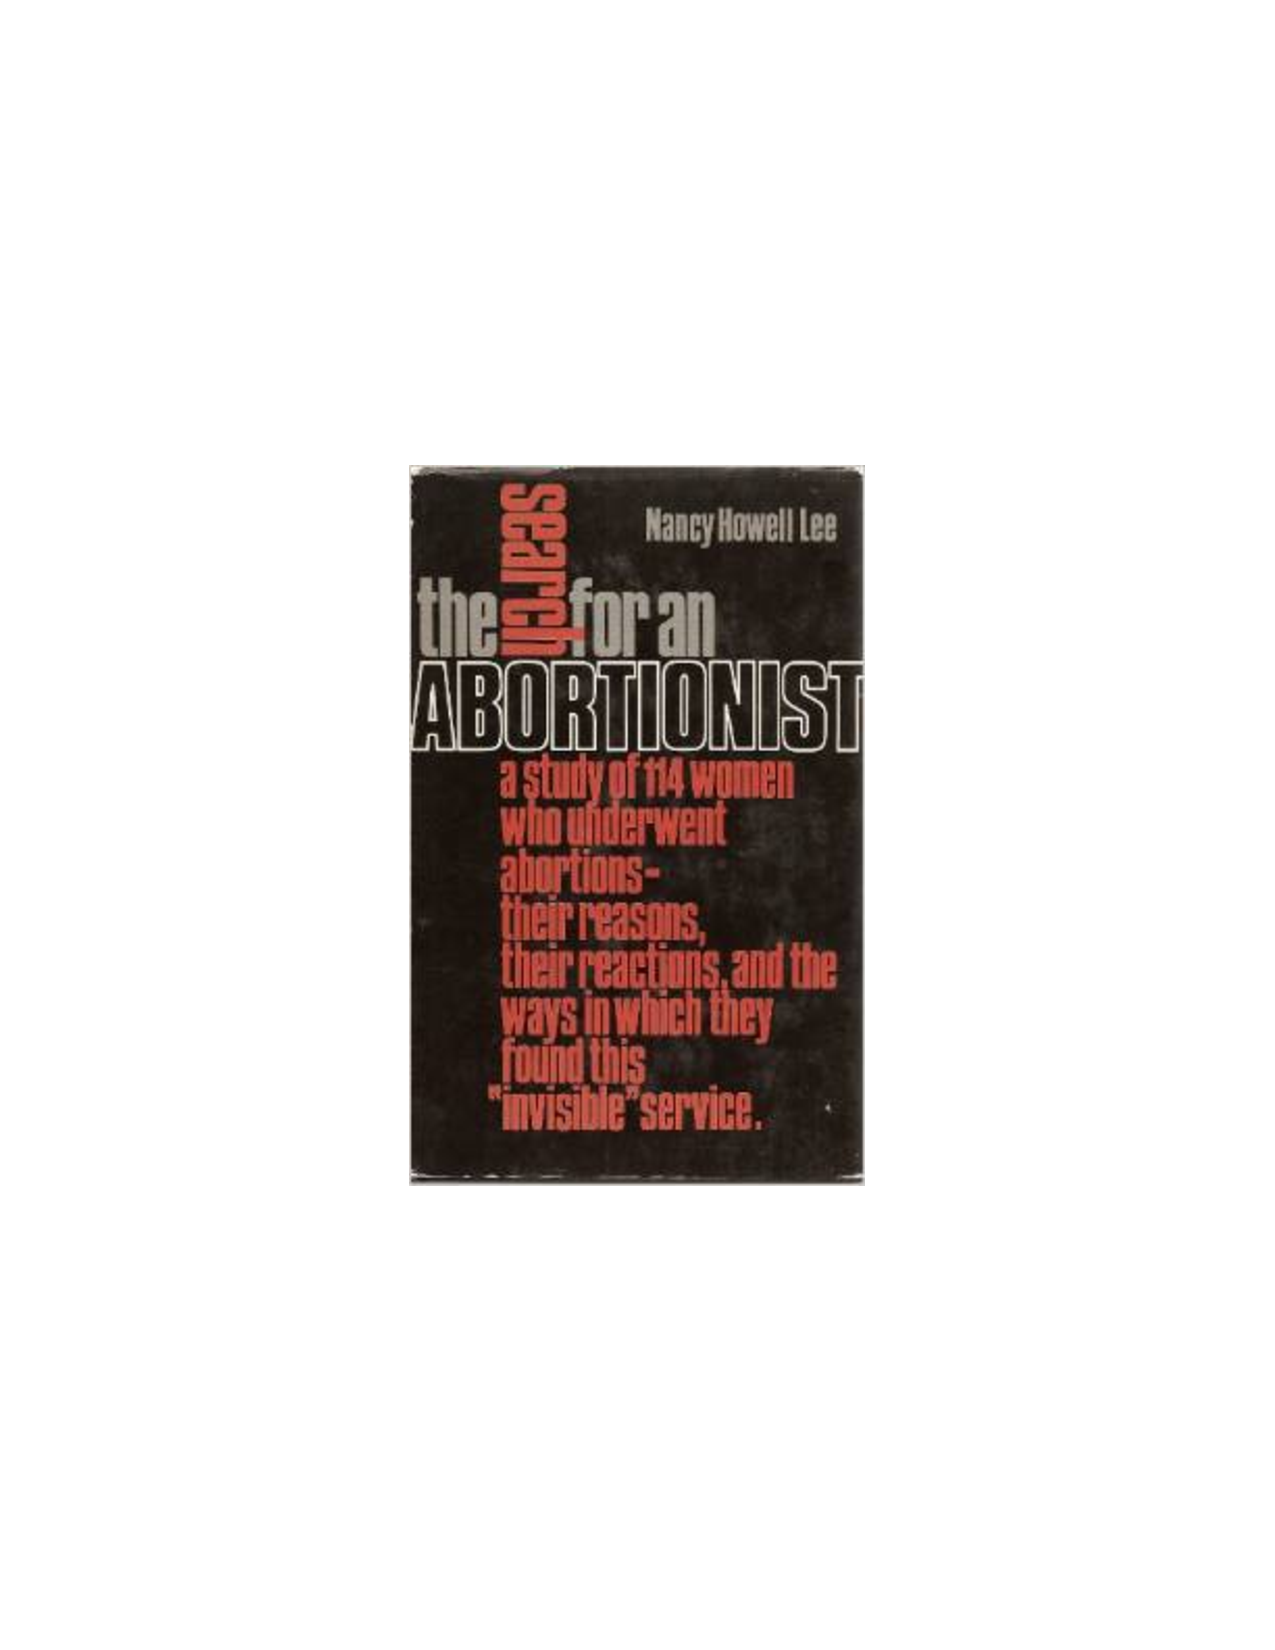
\includegraphics[height=1.3\textheight]{figures/lee_search_1969_cover}
\end{figure}

\note{
Imagine that you are pregnant in 1965 and you want to have an abortion.  Since you cannot search through formal channels (no phone book, no google) the first thing you are probably going to do is ask for help.  Also, you have to remember that this is very time sensitive.  Most doctors didn't want to do an abortion after the 12th week.  Typically searchers had 6 weeks.  Who are you going to ask?  Are they going to help you directly or pass you on to other people?  Which channels will lead to an abolitionist that you trust? to an abortionist you don't trust?  That is what Lee set out to understand.  

Beyond this specific really important application, this study helps us understand search in network more generally.  Remember that one problem in the small world search was attrition.  Here the searchers are very motivated. Also, because this is a such a traumatic period, they are able to recall what they did.  

I want to say that although abortion is a sensitive issue, this is a not a debate about the ethics of abortion.  We are going to discuss an empirical piece of social science.

Work done between 1965 and 67, right around the time Milgram was doing his research (also at Harvard)

Finally, I want to point out the importance of demographic diversity among researchers.  Lee was a woman, and I find it unlikely that a man would have chosen to research this topic even though it was important (and produced fundamental insights).

}

\end{frame}
%%%%%%%%%%%%%%%%%%%%%%%%%%%
\begin{frame}

You didn't read this, but here's some additional background information about study
\begin{itemize}
\item She took great care to protect the confidentiality of participants
\pause
\item She decided not to interview people with failed searches (and she talked about how this might impact her results)
\pause
\item She had to search for people who searched for an abortionist (and she talked about how this might impact her results)
\end{itemize}

\end{frame}
%%%%%%%%%%%%%%%%%%%%%%%%%%%
\begin{frame}

\begin{figure}
\center
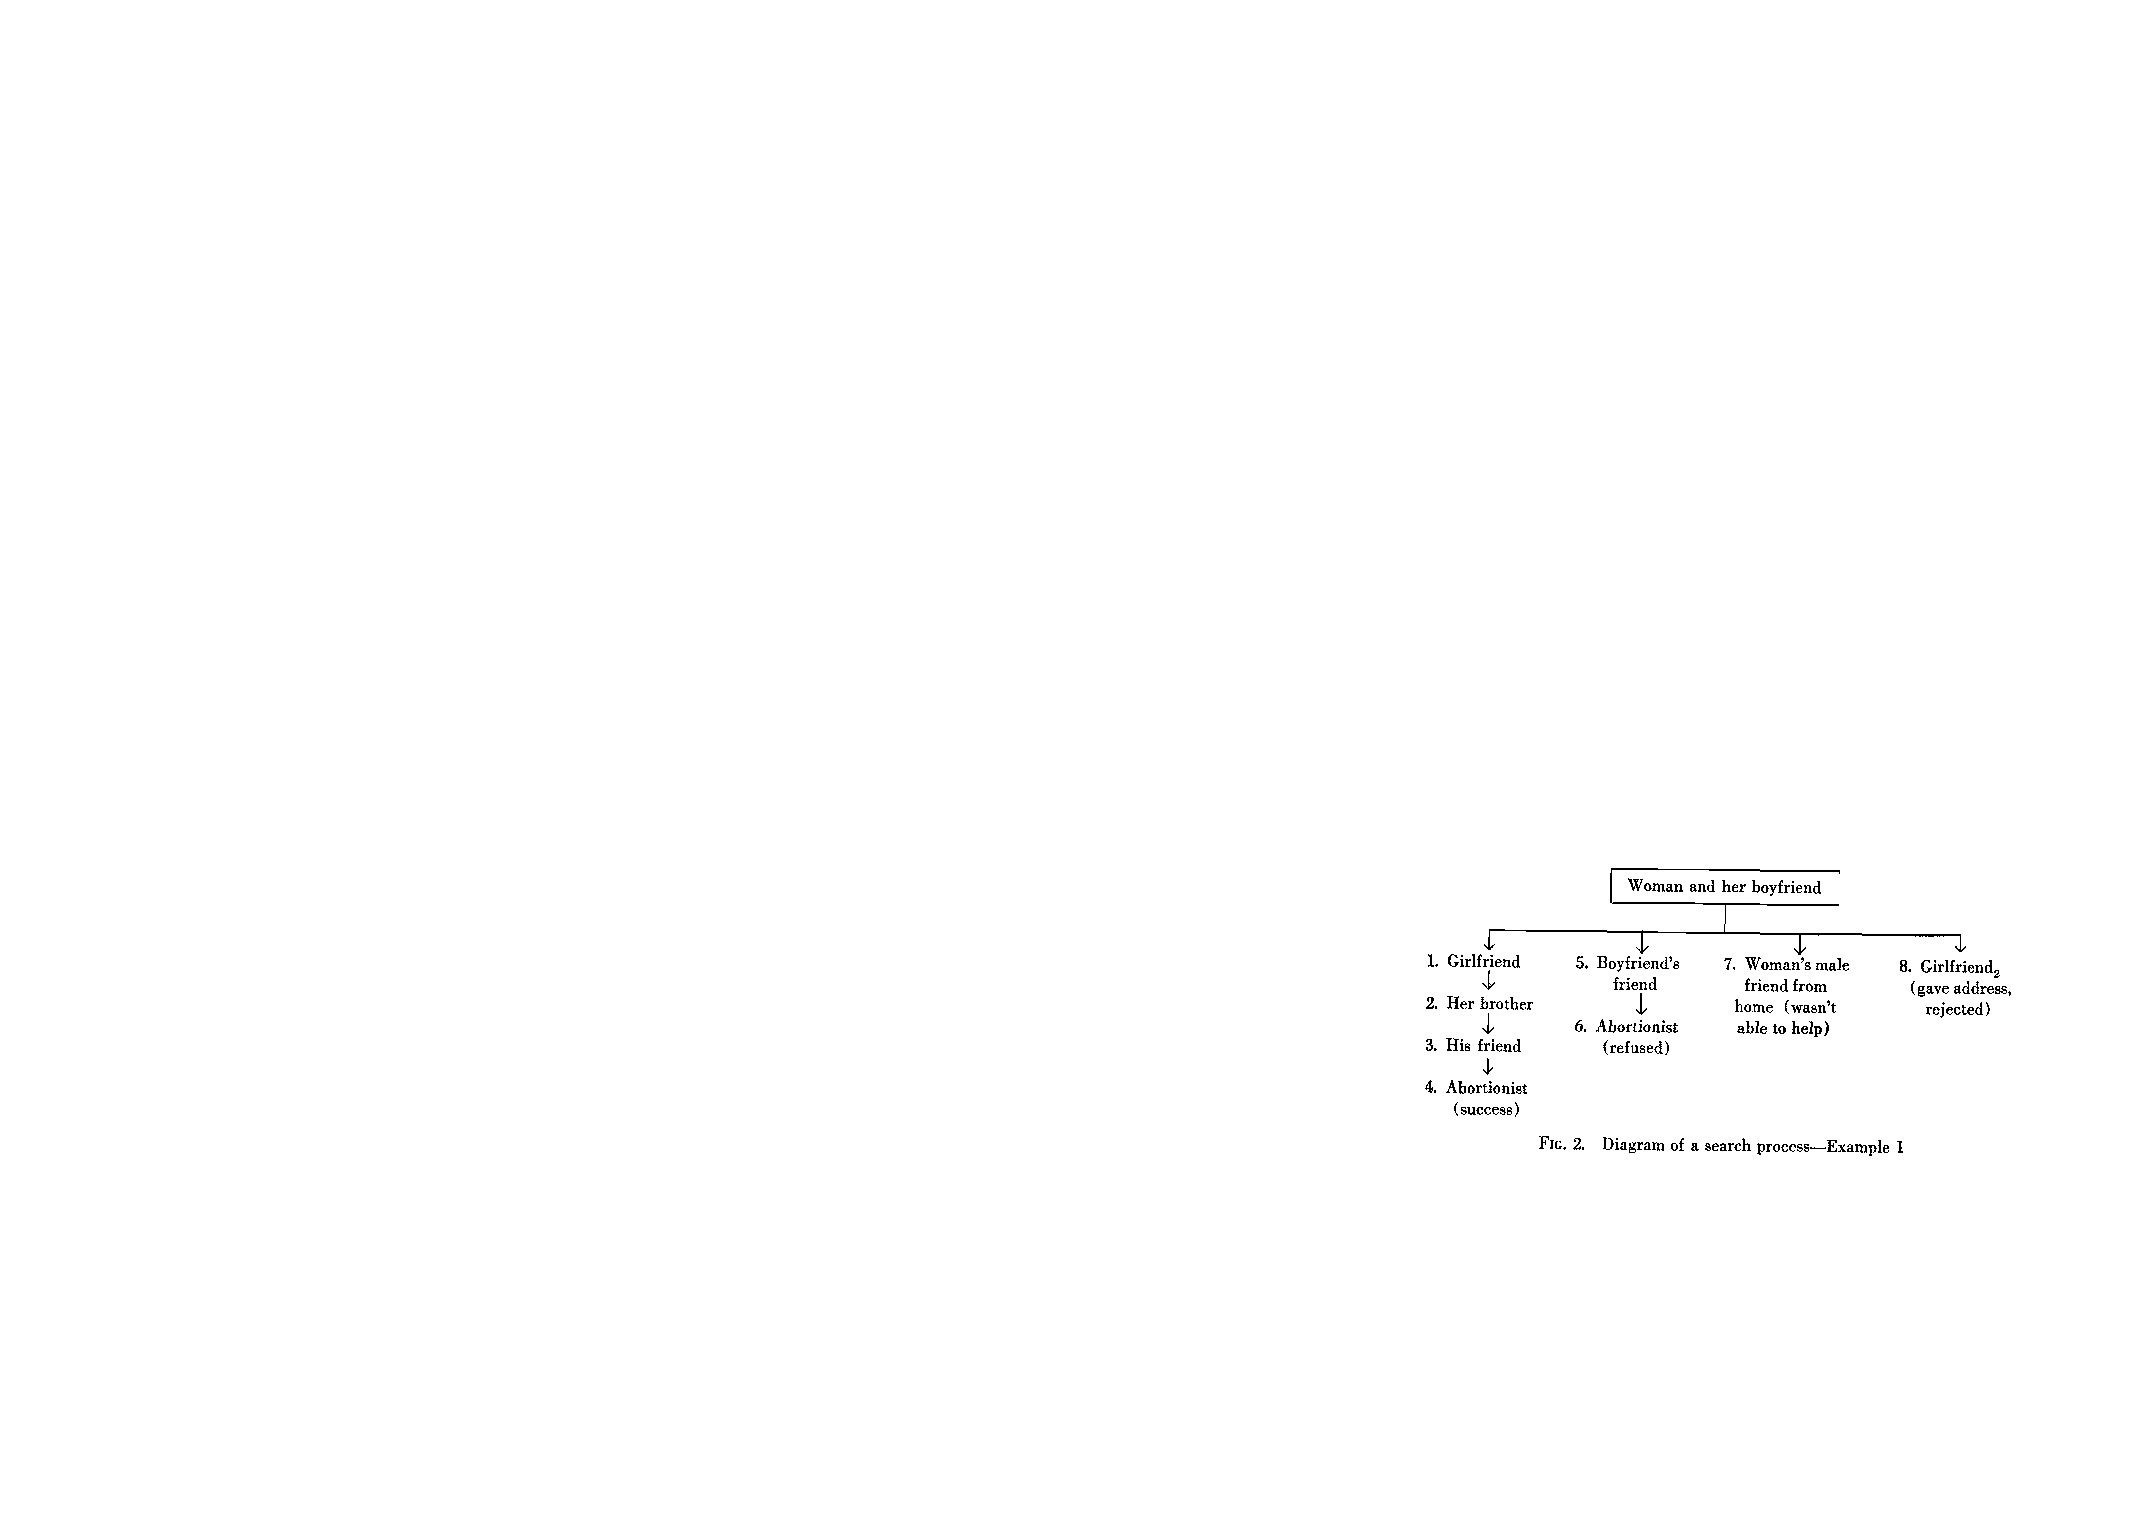
\includegraphics[width = 0.7\textwidth]{figures/lee_search_1969_fig2}
\end{figure}

\pause 
Summary statistics:
\begin{itemize}
\item 8 people involved
\item 4 fresh starts
\item 4 links to abortionist (3 intermediaries)
\end{itemize}


\note{
Here's the story of an 18 year student who was away from home at summer school when she found out that she was pregnant. 

``I asked the girl I was staying with as I knew her brother would probably be able to help.  She was a close friend with whom I had been at school.  She told her brother, who supplied me with an address of a girl who had had an abortion.  I called up the girl who gave the doctor's address.
My boyfriend also obtained an address from another girl, and went to see the doctor.  He was unwilling.
I wrote to a friend (male) at home who could obtain pills for me.  He was unable to do so since the man through whom he could obtain them was away.
I wrote to a girl friend at home who gave me the address of another man, but I was unwilling to report to this method as I had heard it was dangerous.''

This is just 1 of 114 stories.  How did she find people to study (this was not in what you were provided)?  It could be a whole different book on search for research subjects.  She only decided to interview women who had successfully found an abortionist.  Failed searchers were not included because she thought it might be traumatic to talk about attempting to find an abortion for a child that now is alive.  This is sensible, but from a research perspective unfortunate because failed searches would be interesting.  This is similar to the problem of studying ``good'' school.  If you want to learn what makes good schools work well you can go to some good schools and see what they all have in common; for example, bathrooms.  In order to learn about what makes schools good you need to see good schools and bad school.  Unfortunately that is not possible here.\\

She approached birth control clinics, abortionists, political organizations relating to abortion rights, etc.  This lead to a number of leads and also people began to contact here.  She ended up with 25 interviews and 89 surveys for a total of 114 people.

Notice that she does a lot of work to make things standarizable and comparable.  Similar to how Milgram turns a story into a systematic piece of research.

Also note that this is neither pure broadcast or pure directed
}

\end{frame}
%%%%%%%%%%%%%%%%%%%%%%%%%%%
\begin{frame}

\begin{figure}
\center
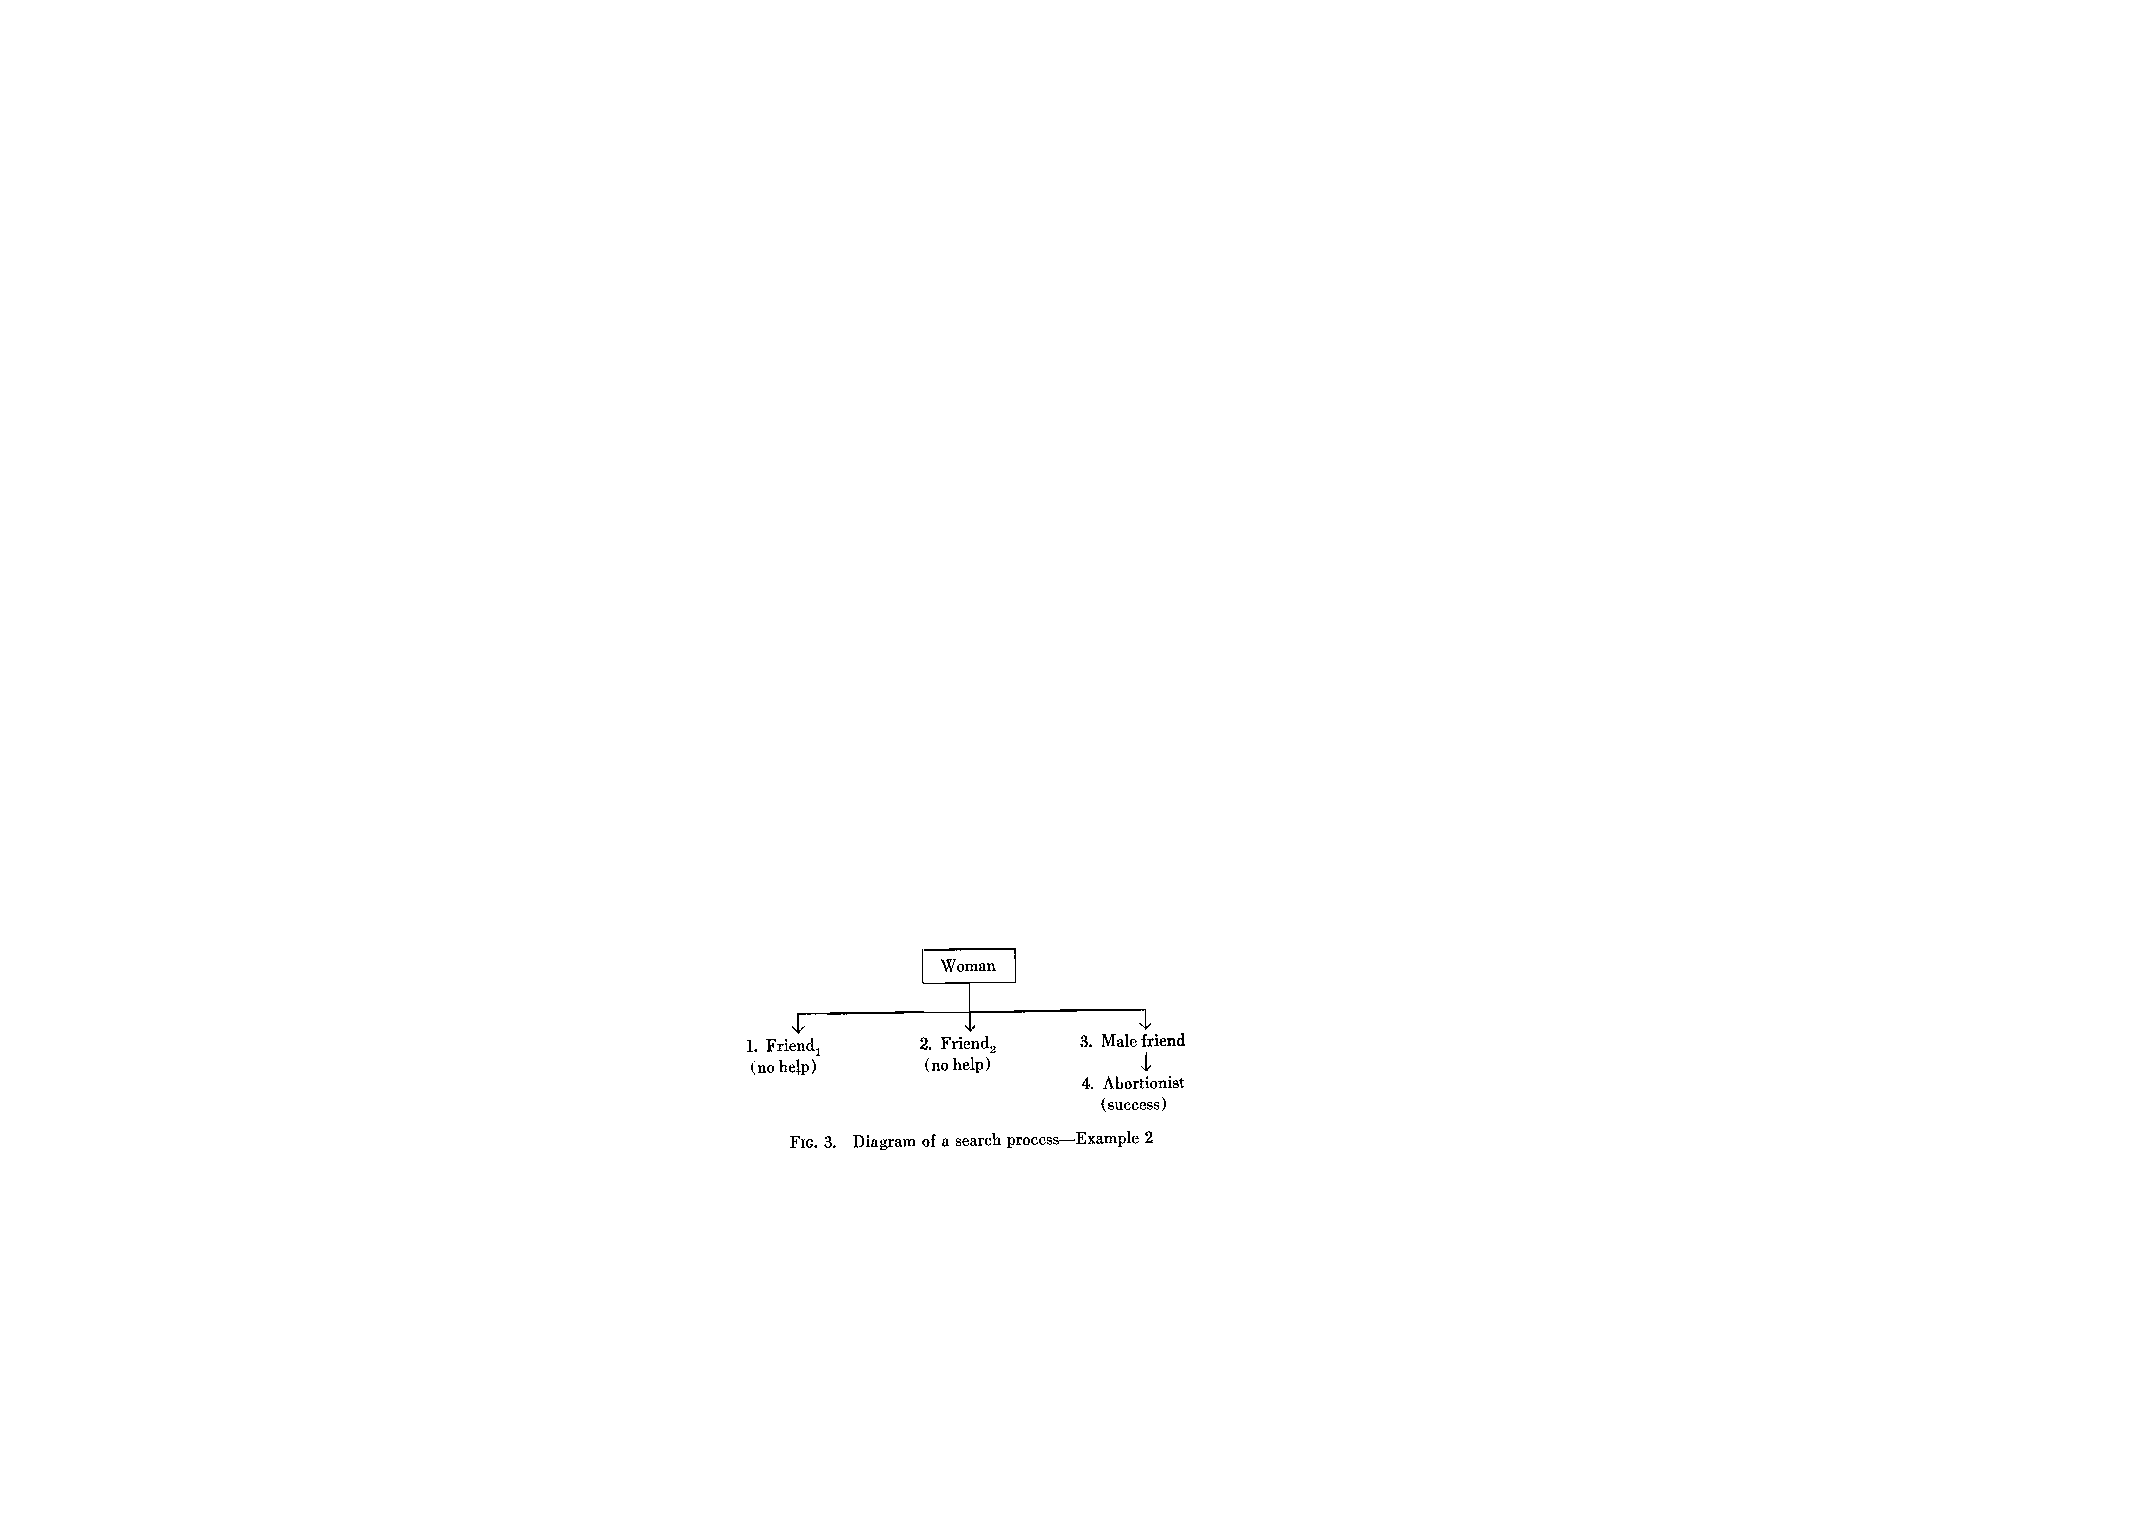
\includegraphics[width = 0.5\textwidth]{figures/lee_search_1969_fig3}
\end{figure}

\pause
Summary statistics:
\begin{itemize}
\item people involved: \onslide<3-5>{4}
\item fresh starts: \onslide<4-5>{3}
\item links to abortionist: \onslide<5>{2}
\end{itemize}


\note{
Here's the story of a 20 year old woman who got pregnant with a man she barely know.
\begin{quote}
I told my two roommates because they were my closest friends and because my parents would have been shocked and unable to have understood.  They had no advice but agreed with my idea of abortion.
I told a close male friend---asked him because of previous conversations (knew he know of a contact with an abortionist).  He gave me the name and number to call and reassurance that previous abortions this man had preformed had not results in any complications.  I also had confidence that our discussion would be confidential.

Note role of trust. Compare to Travers and Milgram.

\end{quote}
}

\end{frame}
%%%%%%%%%%%%%%%%%%%%%%%%%
\begin{frame}

\begin{figure}
\center
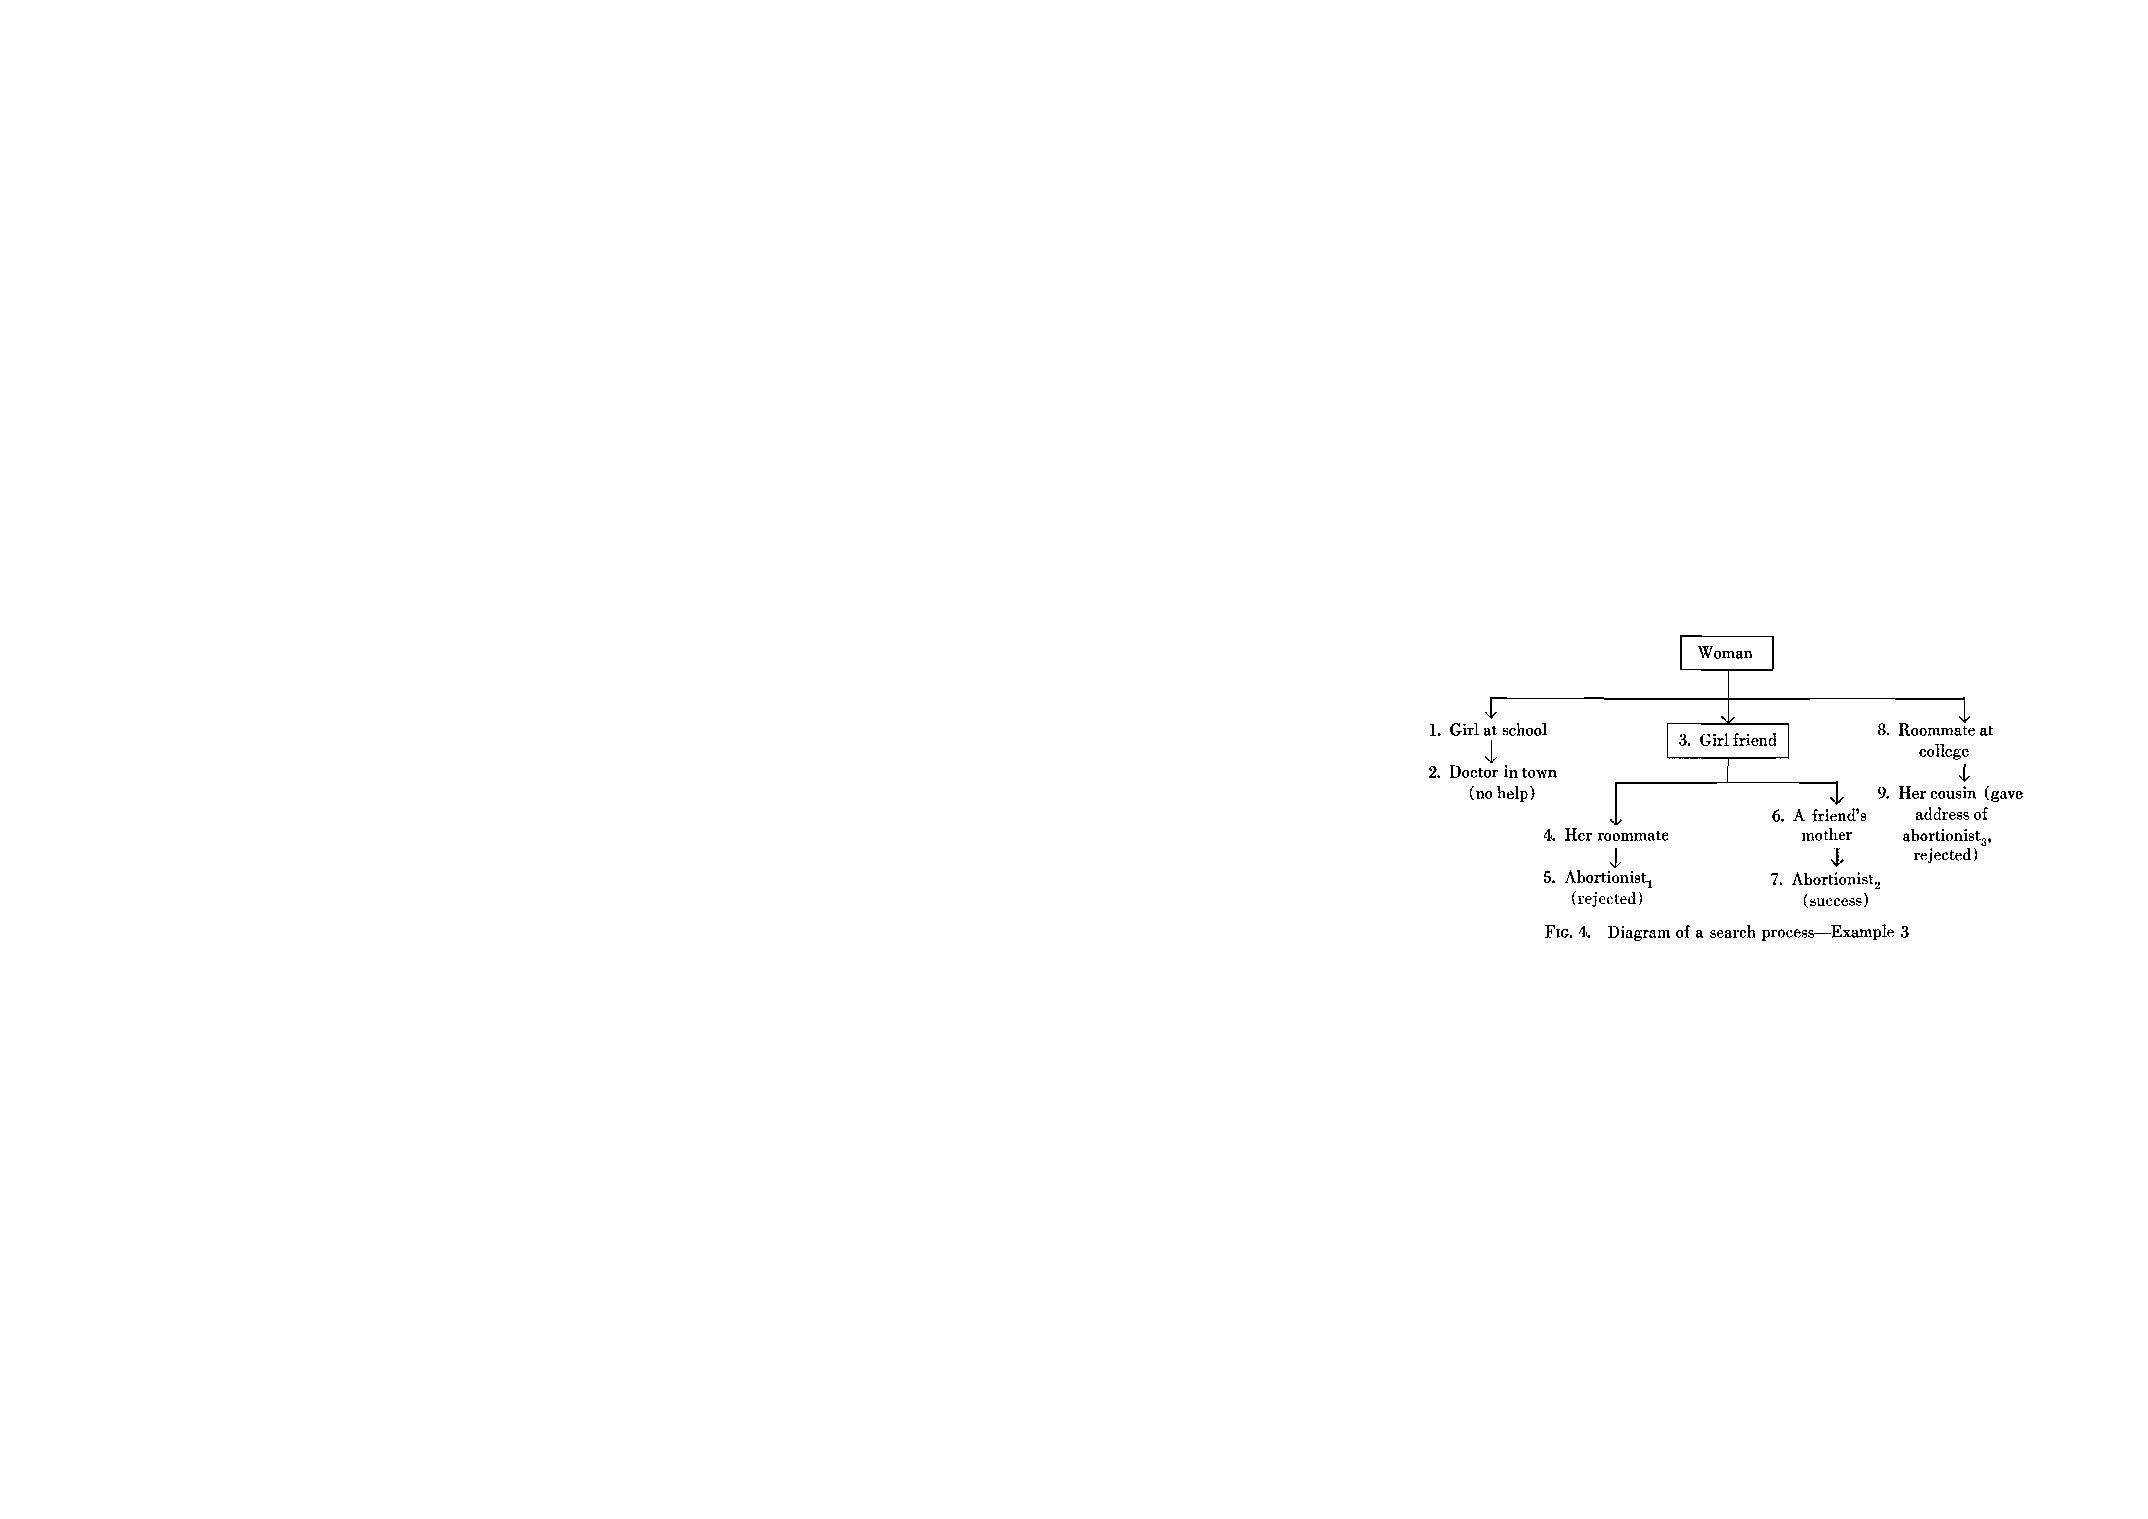
\includegraphics[width = 0.6\textwidth]{figures/lee_search_1969_fig4}
\end{figure}

\pause
Summary statistics:
\begin{itemize}
\item people involved:  \onslide<3-5>{9}
\item fresh starts:  \onslide<4-5>{3}
\item links to abortionist:  \onslide<5>{3}
\end{itemize}

\note{
Here's the story of a women of unspecified age who boyfriend was out of the country when she found out.
``I told this girl at school I was worried, and she lent me her car an told me about a doctor in town who was supposed to be sympathetic.  I went to him for a pregnancy test and I had to back again to get the results, and I asked him what I could do but he said I would have to get married or something.  So I didn't push it.  When the test was positive I call my girl friend (in another city) and told her I was coming to say with her and she should try to find out anything she could.  When I got there she had found out about two people, one guy in the city from her roommate and one out of town from the mother of a friend of ours.  We made an appointment to the see the guy in the city and we went there, but it was so depressing that I had an examinations and said I would come back but I never did.  In the meantime my roommate from college heard about another doctor who was out of town.  We called up and made an appointment, and went to see him.''
}

\end{frame}
%%%%%%%%%%%%%%%%%
\begin{frame}

\begin{figure}
\center
\only<1>{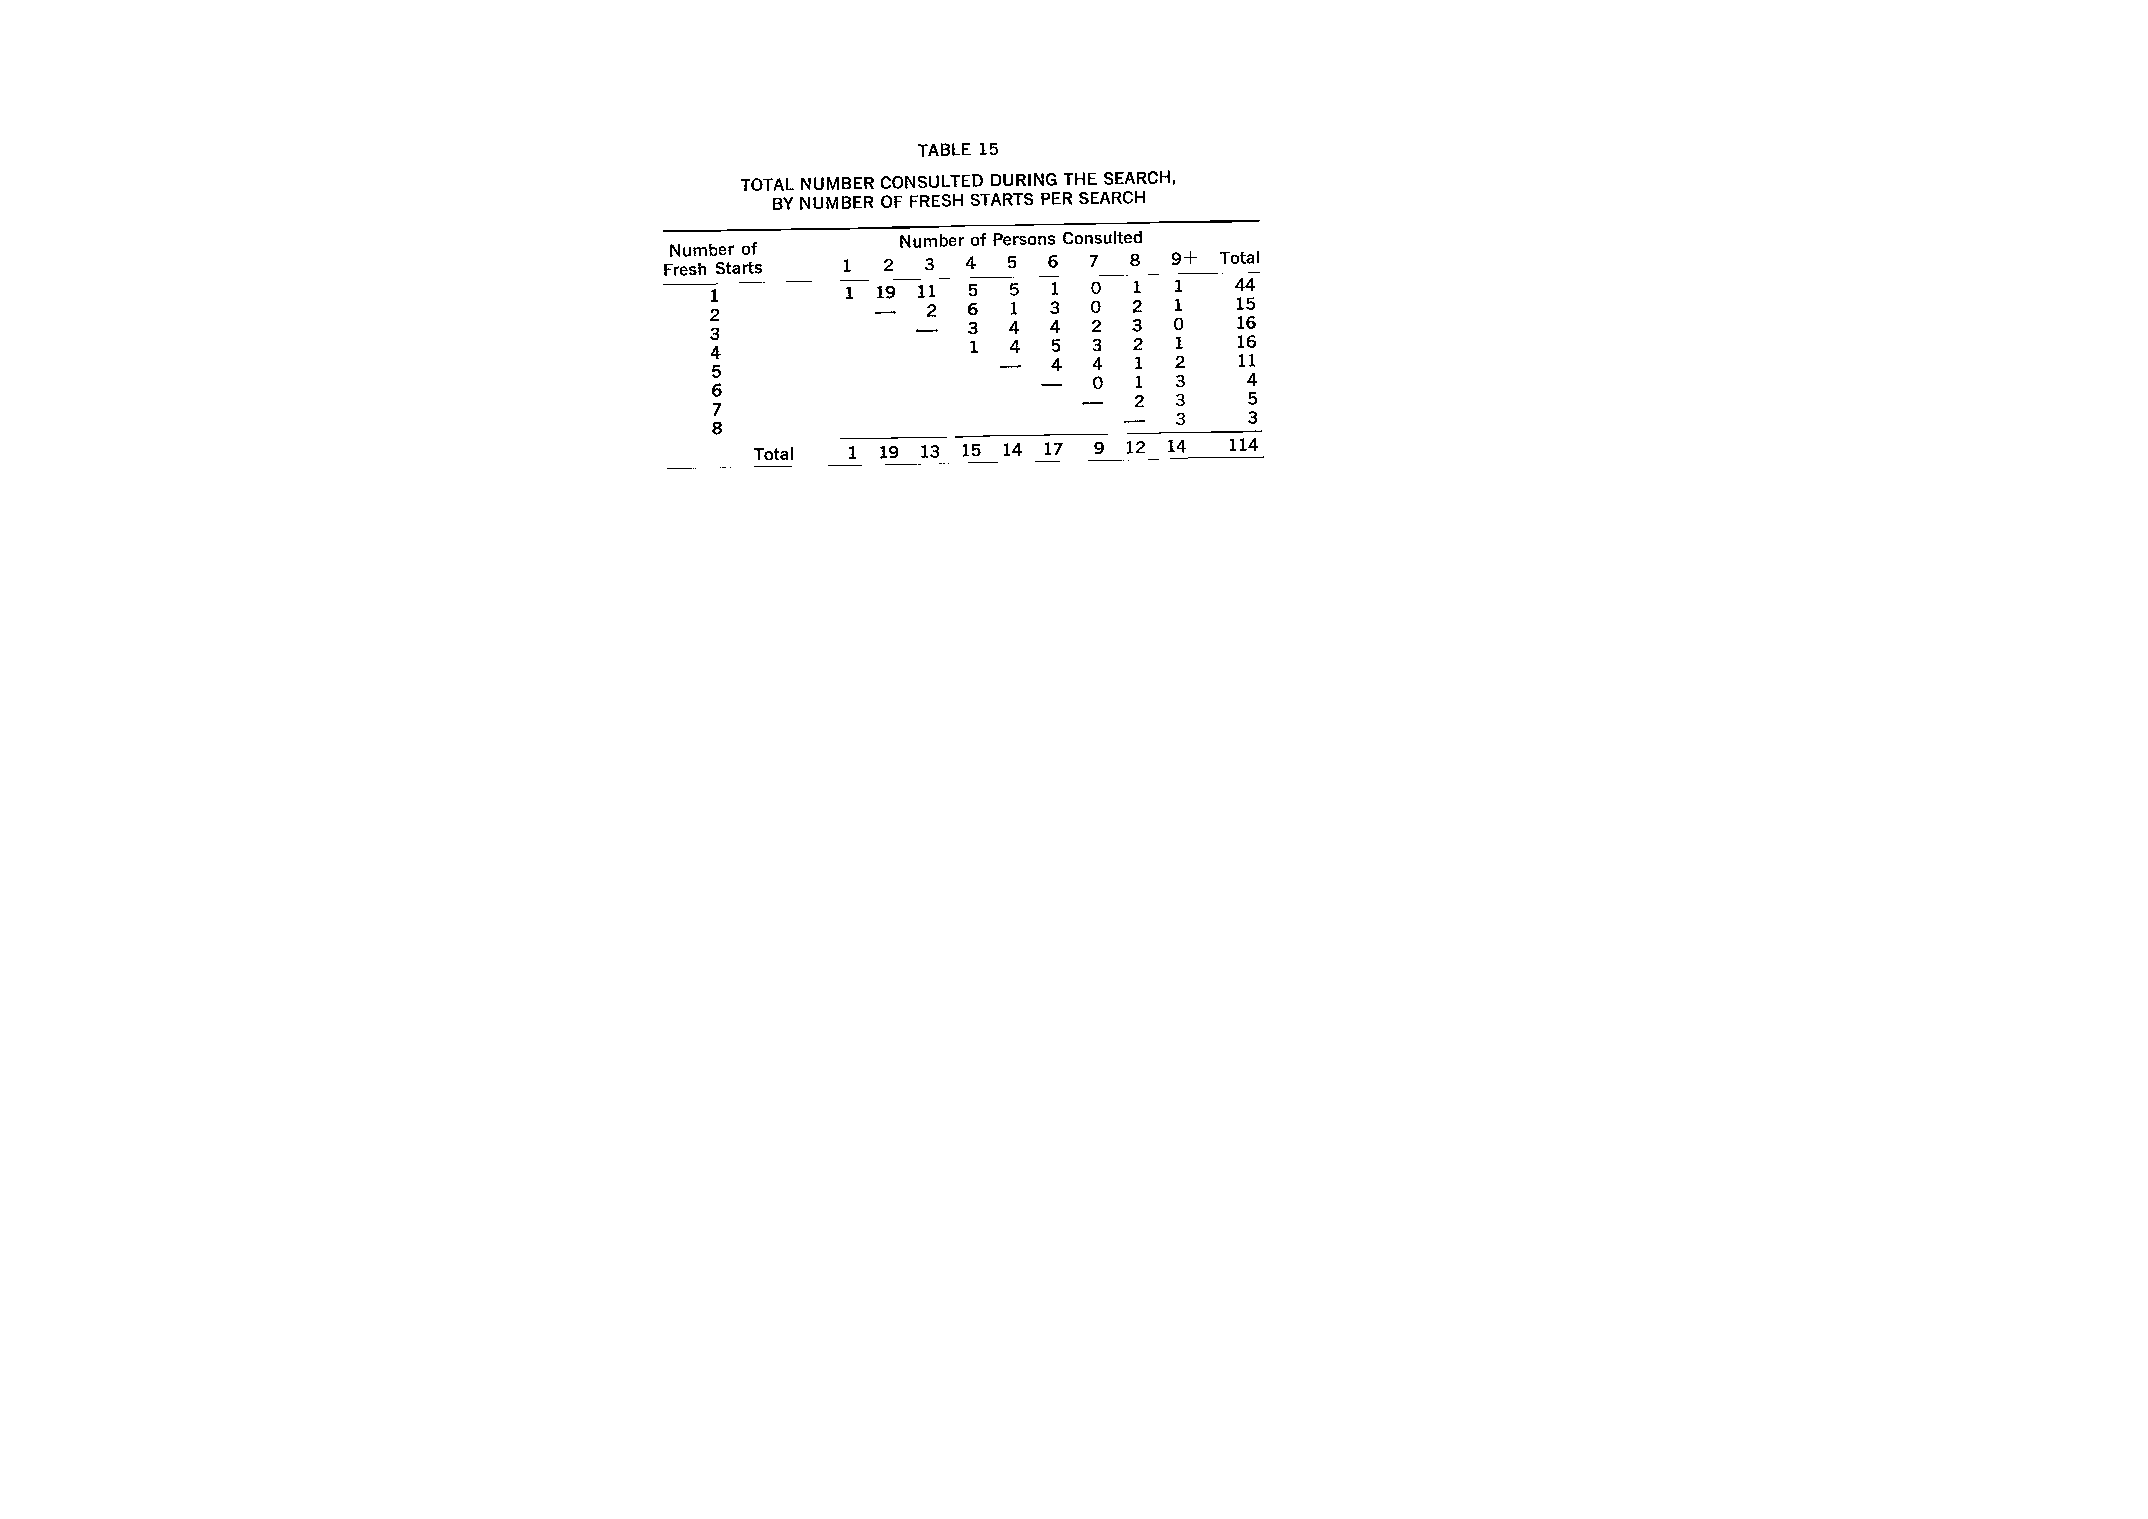
\includegraphics[width = 0.8\textwidth]{figures/lee_search_1969_tab15}}
\only<2>{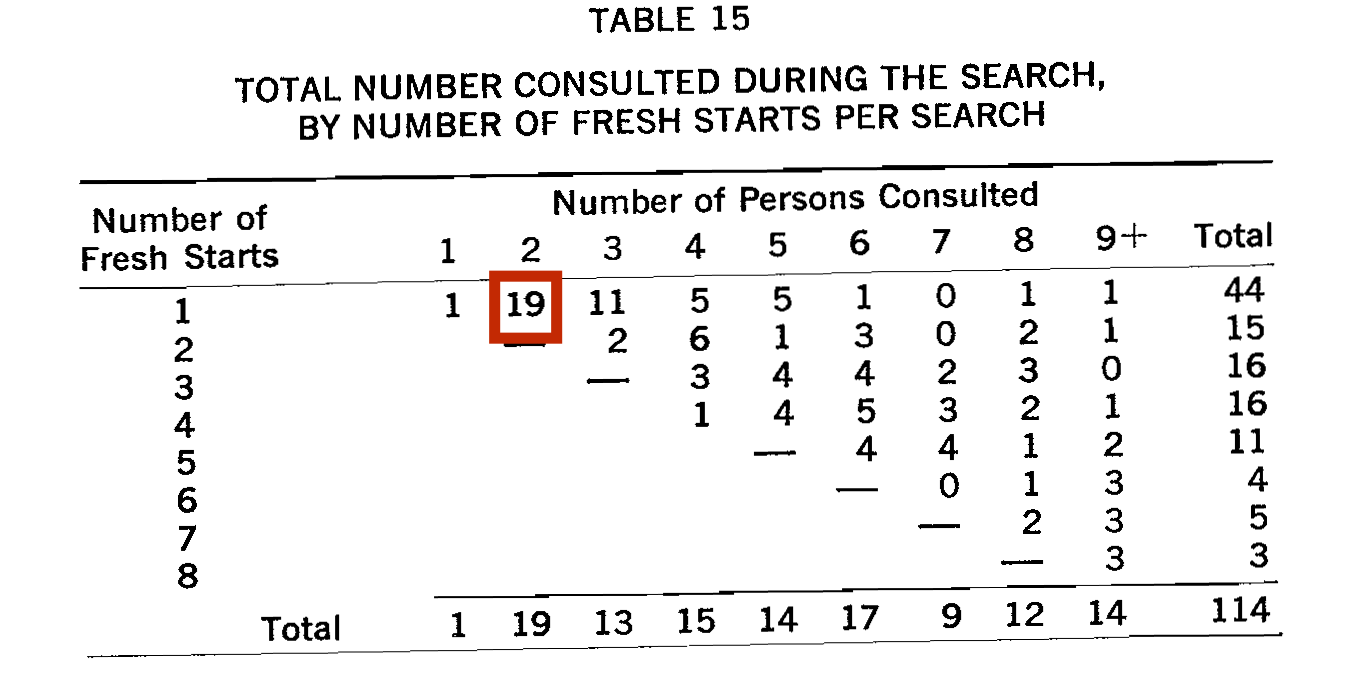
\includegraphics[width = 0.8\textwidth]{figures/lee_search_1969_tab15_19}}
\only<3>{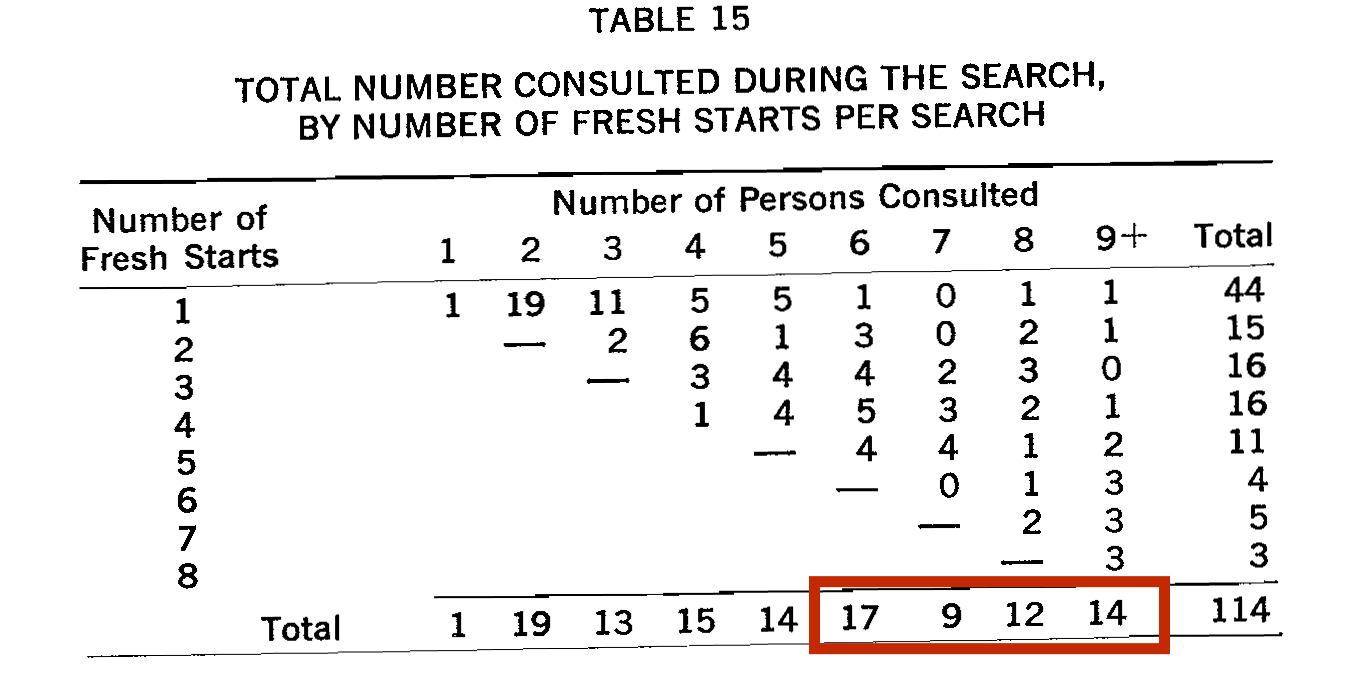
\includegraphics[width = 0.8\textwidth]{figures/lee_search_1969_tab15_bottomrow}}
\end{figure}

\only<2>{In 19 cases, the searchers contacted someone that lead her to an abortionist.}
\only<3>{About half the searches involved 6 or more people.}

\note{
marginals are most interesting
}

\end{frame}
%%%%%%%%%%%%%%%%
\begin{frame}

\begin{figure}
\center
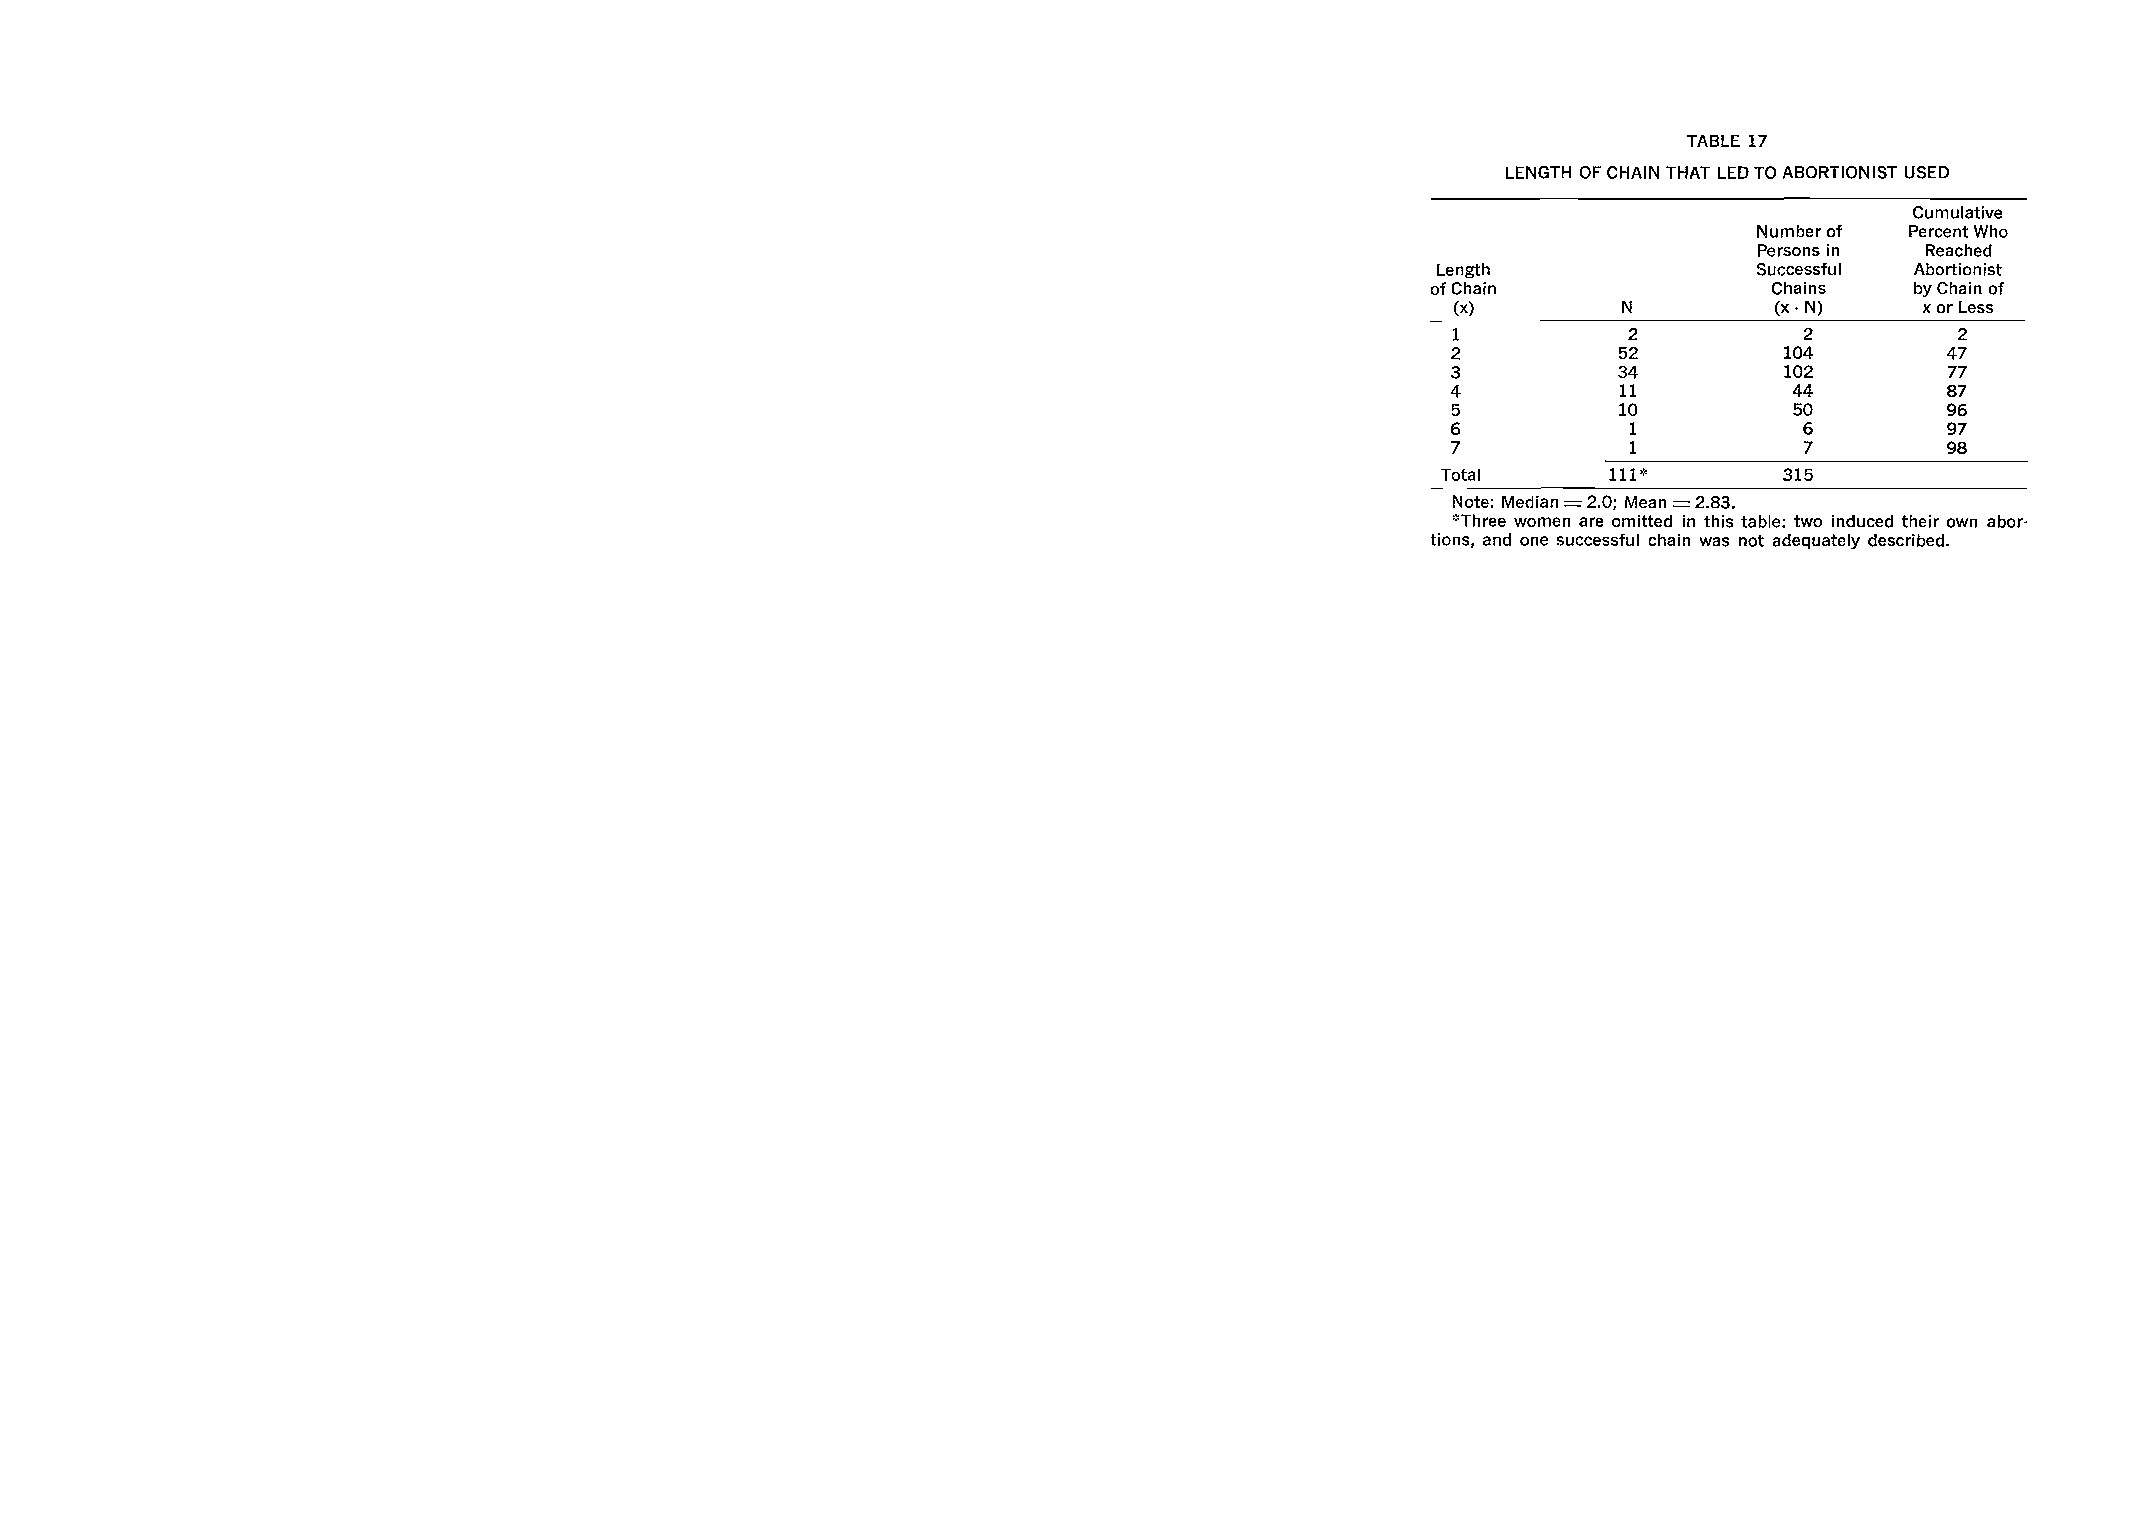
\includegraphics[width = 0.8\textwidth]{figures/lee_search_1969_tab17}
\end{figure}

\pause

Chain length of 2 links was most common

\note{
chain length of 2 was most common
shorter chains might make you most trusting in who you found
}

\end{frame}
%%%%%%%%%%%%%%%%
\begin{frame}

\begin{figure}
\center
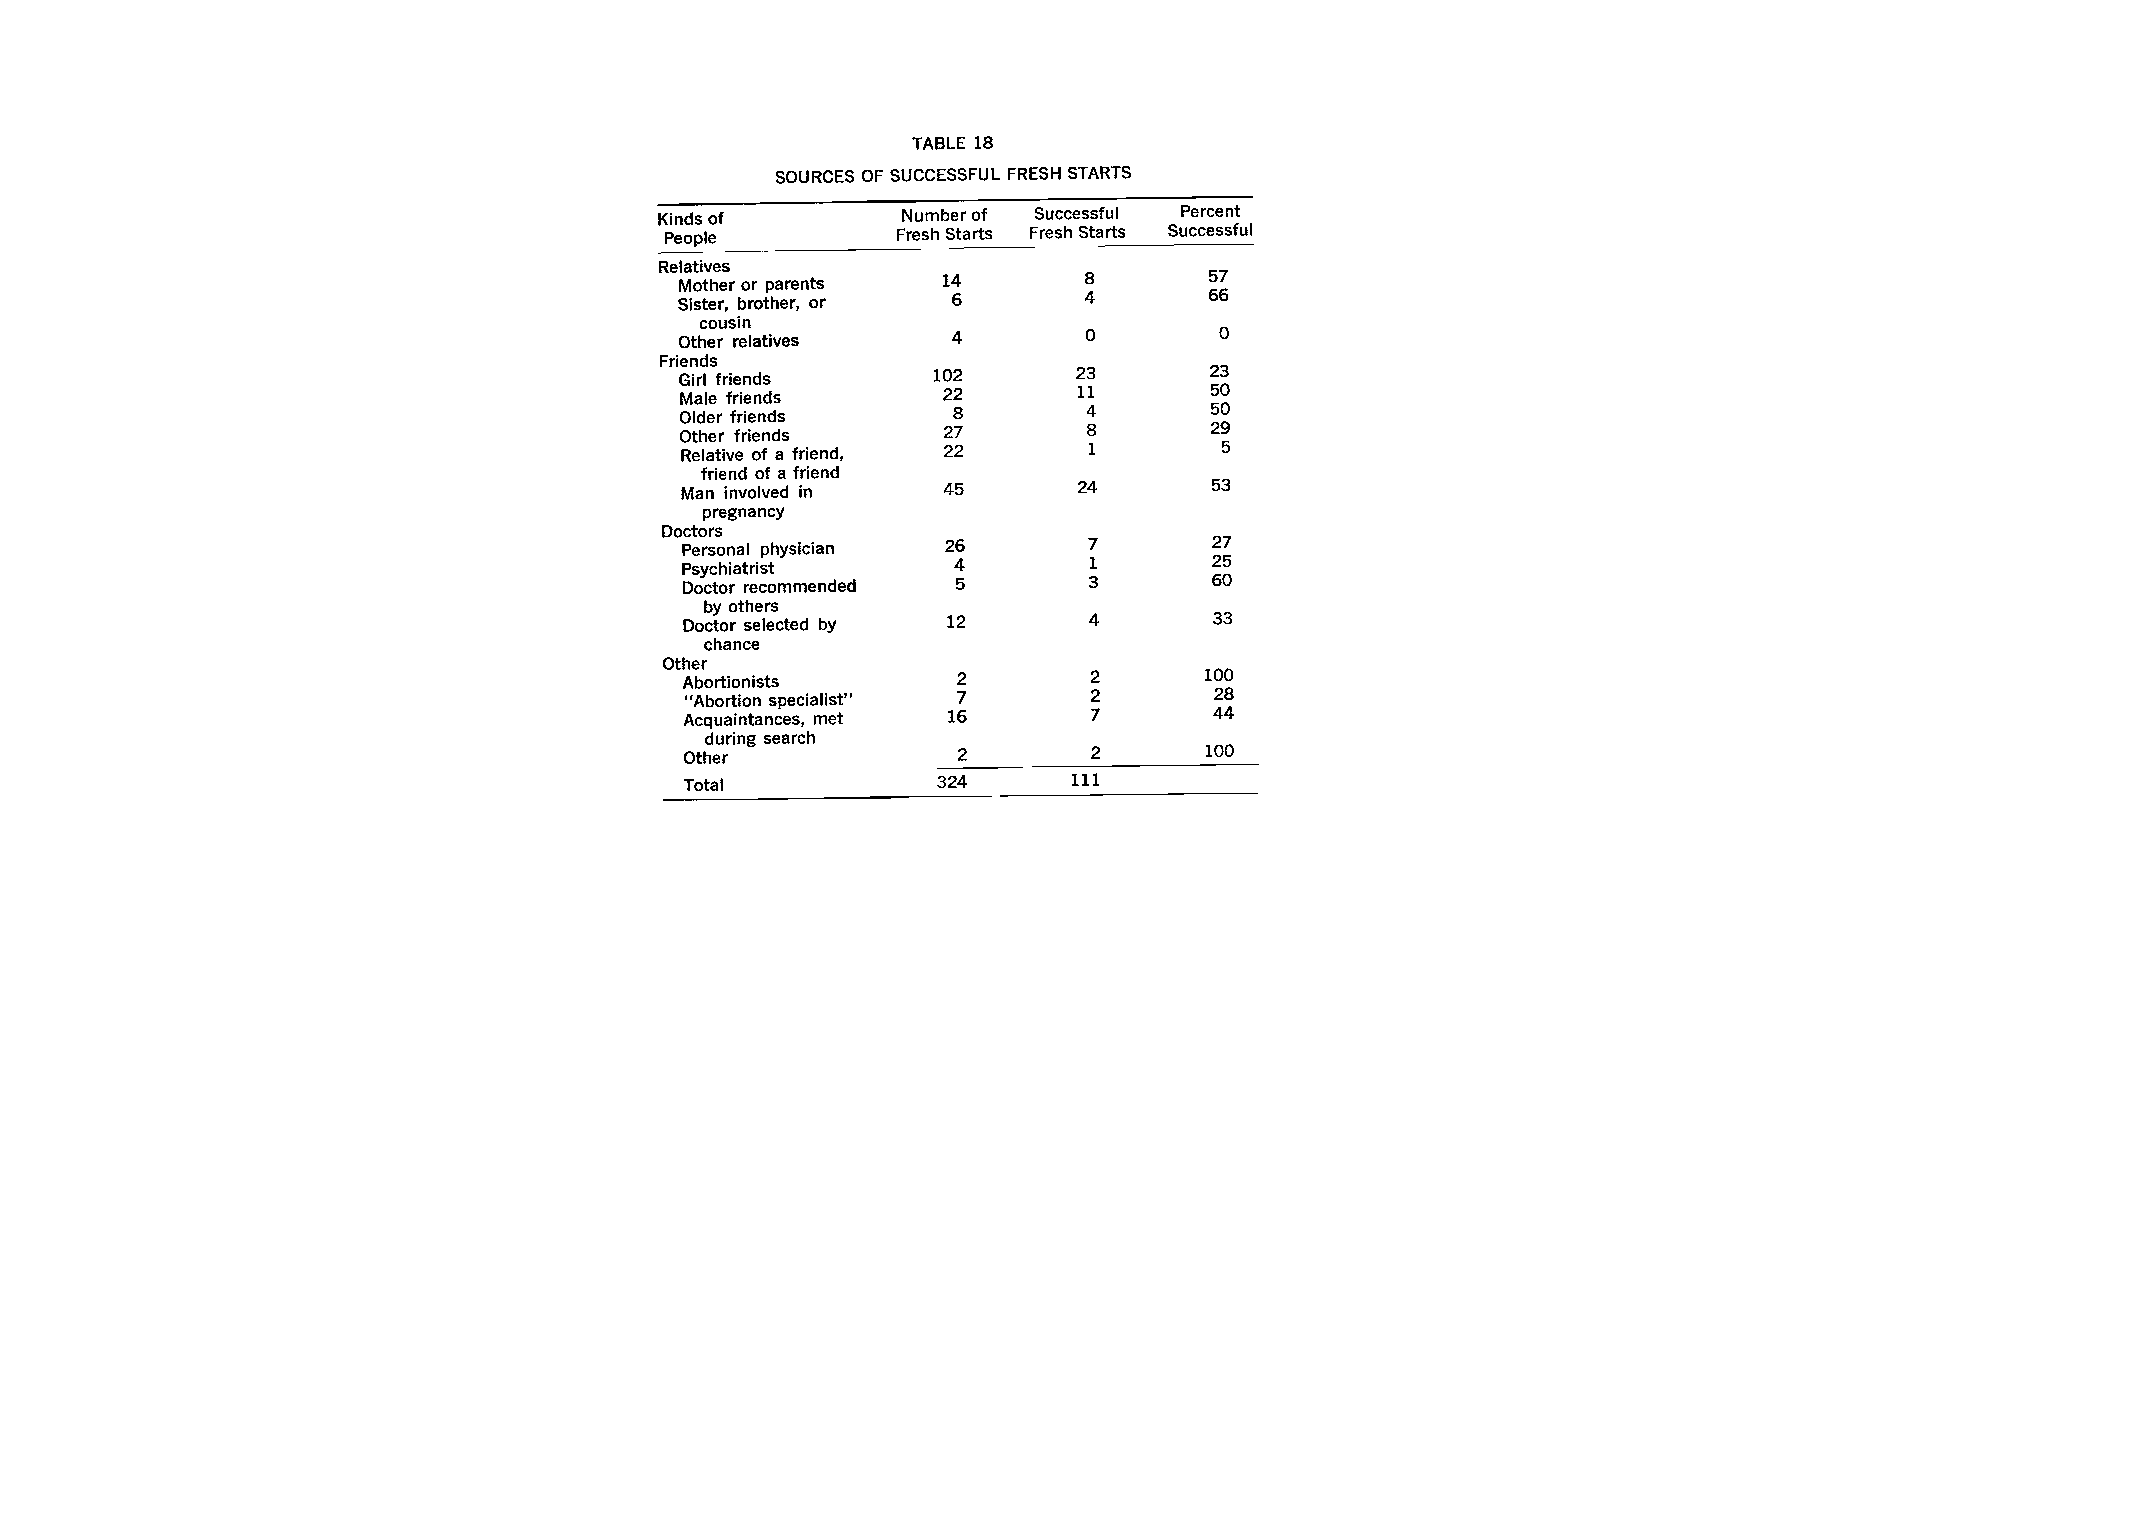
\includegraphics[width = 0.5\textwidth]{figures/lee_search_1969_tab18}
\end{figure}

Weak ties might have access to new information but not always very effective, probably because of effort

\note{
weak ties are not always best because of lack of effort
}

\end{frame}
%%%%%%%%%%%%%%%%
\begin{frame}

\begin{figure}
\center

\includegraphics[width = \textwidth]{figures/ott_getting_2013_title}
\end{figure}

\end{frame}
%%%%%%%%%%%%%%%%
\begin{frame}

\begin{itemize}
\item small world experiments show both 1) short paths exist and 2) people can find them with local information
\pause
\item new models explain why social networks might be searchable and how to design searchable networks
\pause
\item examples of directed searches in networks with real consequences
\end{itemize}

\end{frame}
%%%%%%%%%%%%%%%%
\begin{frame}

Turning point in the class:\\
Network structure $\rightarrow$ dynamics on networks

\end{frame}
%%%%%%%%%%%%%%%%
\begin{frame}

Next class
\begin{itemize}
\item  Watts, Chapter 6. (not posted on Canvas)
\item Bearman, P.S., Moody, J.M., and Stovel, K. (2004). Chains of affection: The structure of adolescent romantic and sexual networks. \textit{American Journal of Sociology}.
\end{itemize}

\end{frame}
%%%%%%%%%%%%%%%%%


\end{document}
